\newcommand{\cps}{\frac{\text{cells}}{s}}

\section{Evaluation}\label{sec:evaluation}
We used two metrics to measure the performance of our simulators. First, we
measured the number of cells our simulators can process in one second. Second,
we measured the total execution time of our simulator. The cell throughput
metric is desirable because it is not dependent on the size of the underlying
grid being simulated. However, the cells throughput isn't easily interpreted.
Similarly, total execution time is easy to interpret, yet it varies with the
size of the underlying grid. In this section, we evaluate our simulators using
these two metrics.

We developed three shallow water simulators.
\begin{enumerate}
  \item \ttt{vec}.
    Our \ttt{vec} simulator is a vectorized version of the initial unoptimized
    compiler. It includes all the optimizations discussed in
    \secref{vectorization}.

  \item \ttt{block}.
    Our \ttt{block} simulator introduces blocking in addition to vectorization.
    It includes all the optimizations described in \secref{vectorization} and
    \secref{domaindecomp}.

  \item \ttt{opt}.
    Our \ttt{opt} simulator is a fully optimized simulator that includes
    vectorization, blocking, and parallelization. It includes all the
    optimizations described in \secref{vectorization}, \secref{domaindecomp},
    and \secref{parallelization}.
\end{enumerate}

The cell throughput and total execution time of these three simulators and the
release simulator for various values of $nx$ are given in
\figref{final-timing-result1} and \figref{final-timing-result2}. Our \ttt{vec}
simulator performs better than the release simulator for most values of $nx$,
though surprisingly it performs worse for large grids. Our \ttt{block}
simulator expectedly performs better than both the release and \ttt{vec}
simulator especially for large values of $nx$. Our \ttt{opt} simulator performs
significantly better than almost all other simulators.

Based on our qualitative and quantitative evaluations, we see that our
\ttt{opt} simulator is able to spread computation very well over multiple
threads. The \ttt{opt} simulator completes 4 times faster on average and
up to 6 times faster than the reference simulator.

\begin{figure}[h]
  \centering
  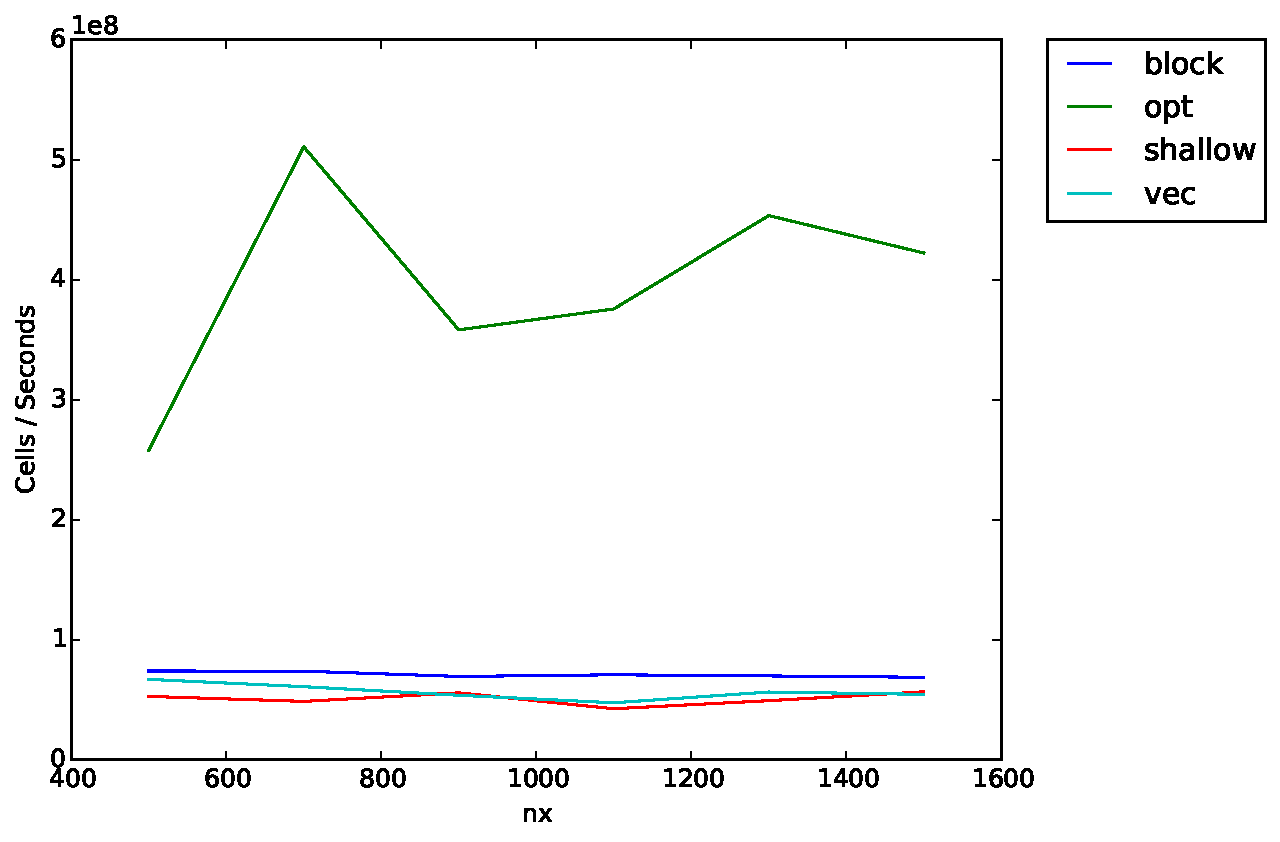
\includegraphics[width=0.8\textwidth]{figs/final-timing1.pdf}
  \caption{Final Timing Result ($cells/seconds$ vs. $nx$)}
  \label{fig:final-timing-result1}
\end{figure}

\begin{figure}[h]
  \centering
  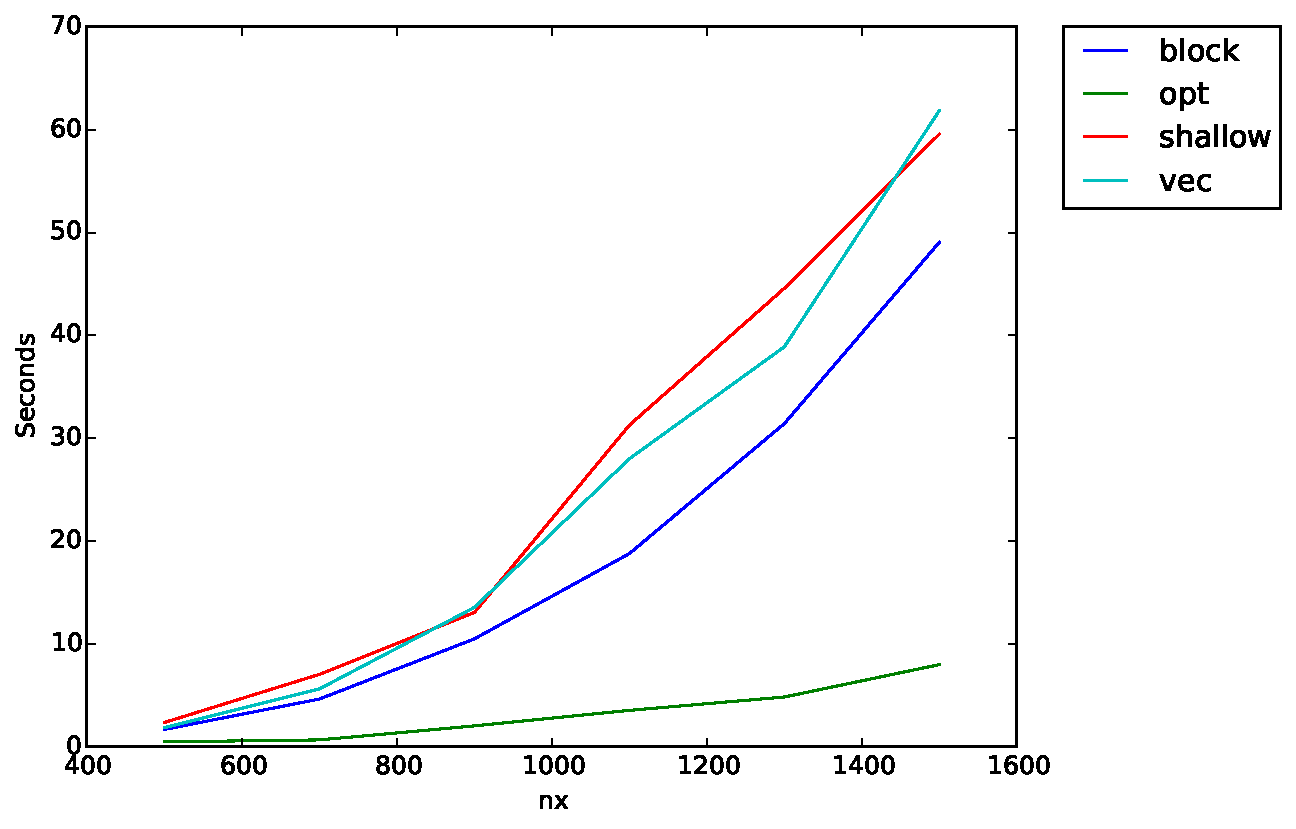
\includegraphics[width=0.8\textwidth]{figs/final-timing2.pdf}
  \caption{Final Timing Result ($seconds$ vs. $nx$)}
  \label{fig:final-timing-result2}
\end{figure}
